\documentclass[10pt]{beamer}
\usepackage[english]{babel}
\usepackage[utf8]{inputenc}
\usepackage[T1]{fontenc}
\usepackage{helvet}

%-------------------------------------------------------
% INFORMATION IN THE TITLE PAGE
%-------------------------------------------------------

\newcommand{\cstitle}{\textbf{ Principales estrategias y métodos basados en deep learning para la detección de neo antígenos en el marco del desarrollo de vacunas personalizadas en la inmunoterapia del cáncer }}
\subtitle[]{Proyecto interno en colaboración con la UCSP}
\newcommand{\cscourseCode}{Matemáticas discretas II}
\newcommand{\csauthor}{PhD(c). Vicente Machaca Arceda \\ PhD. Yván Tupac}
\institute[UNSA]{Universidad de Ingeniería y Tecnología}
\newcommand{\csemail}{vmachaca@utec.edu.pe}
\newcommand{\instituteabr}{UTEC}
\newcommand{\nameUp}{}
\date{2022-I}
\title[\cscourseCode]{\cstitle}
\author{\csauthor}
%%%%%%%%%%%%%%%%%

%-------------------------------------------------------
% CHOOSE THE THEME
%-------------------------------------------------------
\def\mycmd{0} % UNSA
\def\mycmd{1} % SALLE
\def\mycmd{2} % UTEC
\def\mycmd{3} % SALLE NEW
%-------------------------------------------------------

\if\mycmd0
\usepackage{csformat}
\newcommand{\chref}[3][blue]{\href{#2}{\color{#1}{#3}}}%

\fi

\if\mycmd1
\usetheme[]{Feather}
\newcommand{\chref}[2]{	\href{#1}{{\usebeamercolor[bg]{Feather}#2}} }
\fi

\if\mycmd2
\usetheme{UTEC2020}	
\newcommand{\chref}[3][blue]{\href{#2}{\color{#1}{#3}}}%
\fi

\if\mycmd3
\usetheme[]{SALLE}
\newcommand{\chref}[2]{	\href{#1}{{\usebeamercolor[bg]{Feather}#2}} }
\fi


\newcommand{\1}{
	\setbeamertemplate{background}{
		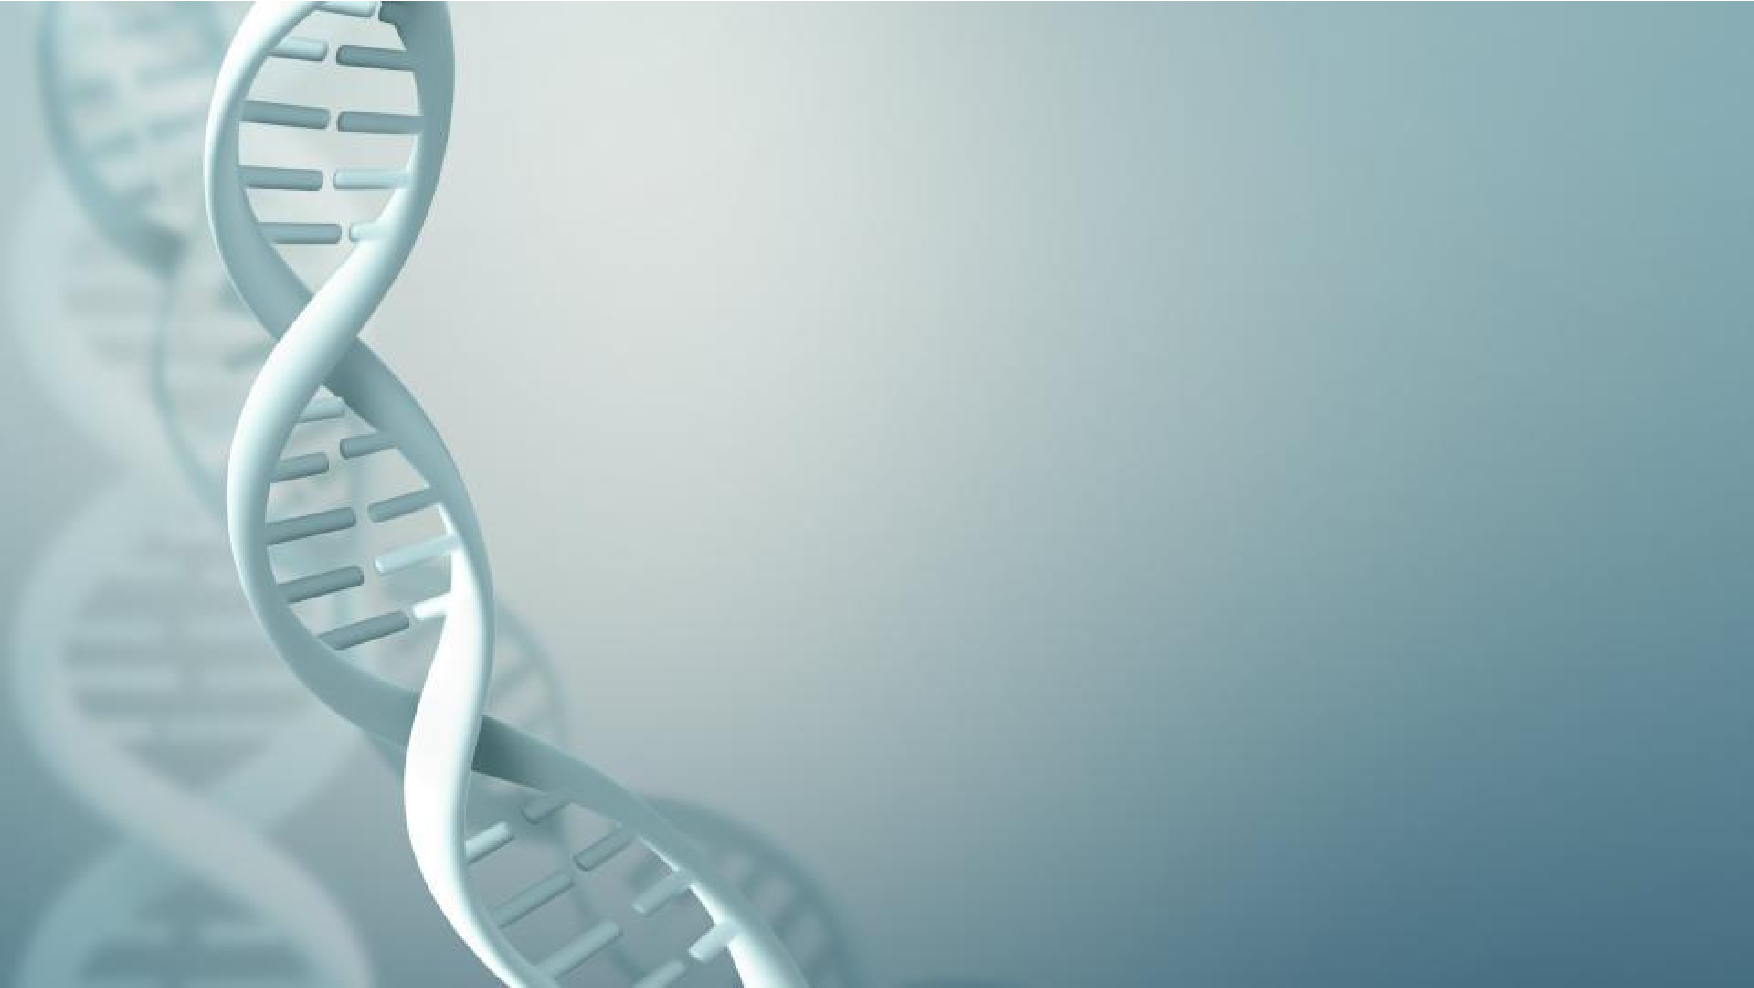
\includegraphics[width=\paperwidth,height=\paperheight]{img/1}
		\tikz[overlay] \fill[fill opacity=0.75,fill=white] (0,0) rectangle (-\paperwidth,\paperheight);
	}
}



%-------------------------------------------------------
% THE BODY OF THE PRESENTATION
%-------------------------------------------------------

\begin{document}
	
	
	\AtBeginSection[]
	{
		\begin{frame}
			\frametitle{Contenido}
			\tableofcontents[currentsubsection]
		\end{frame}
	}
	
	
	%-------------------------------------------------------
	% THE TITLEPAGE
	%-------------------------------------------------------
	
	\if\mycmd0
	\maketitle
	\fi
	
	\if\mycmd1 % MY THEME
	\1{
		\begin{frame}[plain,noframenumbering] 
			\titlepage 
	\end{frame}}
	\fi
	
	\if\mycmd2
	\begin{frame}
		\titlepage
	\end{frame}
	\fi
	
	\if\mycmd3
	%\titlepage
	\begin{frame}[plain,noframenumbering] 
		\titlepage
	\end{frame}
	\fi
	%-------------------------------------------------------
	%-------------------------------------------------------


%-------------------------------------------------------
%-------------------------------------------------------
\begin{frame}{Contenido}
	\tableofcontents
\end{frame}
%-------------------------------------------------------
%-------------------------------------------------------



%%%%%%%%%%%%%%%%%%%%%%%%%%%%%%%%%%%%%%%%%%%%%%%%%%%%%%%%%%%%%%%%%%%%%%%%%%%%%%%%%%%%%%%%%%%%%%%%%%%%%%%%%%%%%%%%
%%%%%%%%%%%%%%%%%%%%%%%%%%%%%%%%%%%%%%%%%%%%%%%%%%%%%%%%%%%%%%%%%%%%%%%%%%%%%%%%%%%%%%%%%%%%%%%%%%%%%%%%%%%%%%%%
%%%%%%%%%%%%%%%%%%%%%%%%%%%%%%%%%%%%%%%%%%%%%%%%%%%%%%%%%%%%%%%%%%%%%%%%%%%%%%%%%%%%%%%%%%%%%%%%%%%%%%%%%%%%%%%%
\section{Introducción}
%%%%%%%%%%%%%%%%%%%%%%%%%%%%%%%%%%%%%%%%%%%%%%%%%%%%%%%%%%%%%%%%%%%%%%%%%%%%%%%%%%%%%%%%%%%%%%%%%%%%%%%%%%%%%%%%
%%%%%%%%%%%%%%%%%%%%%%%%%%%%%%%%%%%%%%%%%%%%%%%%%%%%%%%%%%%%%%%%%%%%%%%%%%%%%%%%%%%%%%%%%%%%%%%%%%%%%%%%%%%%%%%%
%%%%%%%%%%%%%%%%%%%%%%%%%%%%%%%%%%%%%%%%%%%%%%%%%%%%%%%%%%%%%%%%%%%%%%%%%%%%%%%%%%%%%%%%%%%%%%%%%%%%%%%%%%%%%%%%

%%%%%%%%%%%%%%%%%%%%%%%%%%%%%%%%%%%%%%%%%%%%%%%%%%%%%%%%%%%%%%%%%%%%%%%%%%%%%%%%%%%%%%%%%%%%%%%%%%%%%%%%%%%%%%%%
%%%%%%%%%%%%%%%%%%%%%%%%%%%%%%%%%%%%%%%%%%%%%%%%%%%%%%%%%%%%%%%%%%%%%%%%%%%%%%%%%%%%%%%%%%%%%%%%%%%%%%%%%%%%%%%%
%%%%%%%%%%%%%%%%%%%%%%%%%%%%%%%%%%%%%%%%%%%%%%%%%%%%%%%%%%%%%%%%%%%%%%%%%%%%%%%%%%%%%%%%%%%%%%%%%%%%%%%%%%%%%%%%
\subsection{Proyecto}
%%%%%%%%%%%%%%%%%%%%%%%%%%%%%%%%%%%%%%%%%%%%%%%%%%%%%%%%%%%%%%%%%%%%%%%%%%%%%%%%%%%%%%%%%%%%%%%%%%%%%%%%%%%%%%%%
%%%%%%%%%%%%%%%%%%%%%%%%%%%%%%%%%%%%%%%%%%%%%%%%%%%%%%%%%%%%%%%%%%%%%%%%%%%%%%%%%%%%%%%%%%%%%%%%%%%%%%%%%%%%%%%%
%%%%%%%%%%%%%%%%%%%%%%%%%%%%%%%%%%%%%%%%%%%%%%%%%%%%%%%%%%%%%%%%%%%%%%%%%%%%%%%%%%%%%%%%%%%%%%%%%%%%%%%%%%%%%%%%

%-------------------------------------------------------
%-------------------------------------------------------
\begin{frame}{Proyecto}{Financiamiento}		
	\begin{columns}
		\begin{column}{0.48\textwidth}
			
\includegraphics[width=\textwidth]{img/neoantigen/logo_salle}
		\end{column}
	
		\begin{column}{0.48\textwidth}
			
\includegraphics[width=\textwidth]{img/neoantigen/logo_ucsp}
		\end{column}
	\end{columns}		
\end{frame}
%-------------------------------------------------------
%-------------------------------------------------------

%-------------------------------------------------------
%-------------------------------------------------------
\begin{frame}{Proyecto}{Duración y equipo de trabajo}			
	\begin{block}{}
		\begin{itemize}
			\item Seis (06) meses.
			\item Equipo:
			\begin{itemize}
				\item Vicente Machaca Arceda (ULaSalle).
				\item Valeria Goyzueta (ULaSalle).
				\item Yván Tupac (UCSP).
				\item Maria Cruz (UCSP).				
			\end{itemize}
		\end{itemize}
	\end{block}
\end{frame}
%-------------------------------------------------------
%-------------------------------------------------------


%%%%%%%%%%%%%%%%%%%%%%%%%%%%%%%%%%%%%%%%%%%%%%%%%%%%%%%%%%%%%%%%%%%%%%%%%%%%%%%%%%%%%%%%%%%%%%%%%%%%%%%%%%%%%%%%
%%%%%%%%%%%%%%%%%%%%%%%%%%%%%%%%%%%%%%%%%%%%%%%%%%%%%%%%%%%%%%%%%%%%%%%%%%%%%%%%%%%%%%%%%%%%%%%%%%%%%%%%%%%%%%%%
%%%%%%%%%%%%%%%%%%%%%%%%%%%%%%%%%%%%%%%%%%%%%%%%%%%%%%%%%%%%%%%%%%%%%%%%%%%%%%%%%%%%%%%%%%%%%%%%%%%%%%%%%%%%%%%%
\subsection{Neo antígenos}
%%%%%%%%%%%%%%%%%%%%%%%%%%%%%%%%%%%%%%%%%%%%%%%%%%%%%%%%%%%%%%%%%%%%%%%%%%%%%%%%%%%%%%%%%%%%%%%%%%%%%%%%%%%%%%%%
%%%%%%%%%%%%%%%%%%%%%%%%%%%%%%%%%%%%%%%%%%%%%%%%%%%%%%%%%%%%%%%%%%%%%%%%%%%%%%%%%%%%%%%%%%%%%%%%%%%%%%%%%%%%%%%%
%%%%%%%%%%%%%%%%%%%%%%%%%%%%%%%%%%%%%%%%%%%%%%%%%%%%%%%%%%%%%%%%%%%%%%%%%%%%%%%%%%%%%%%%%%%%%%%%%%%%%%%%%%%%%%%%


%-------------------------------------------------------
%-------------------------------------------------------
\begin{frame}{Inmunoterapia del Cáncer}{}		
	Es un tipo de tratamiento contra el Cáncer que estimula las defensas naturales del cuerpo para combatir el Cáncer \cite{inmunoterapy2022}.
		
	\begin{figure}
		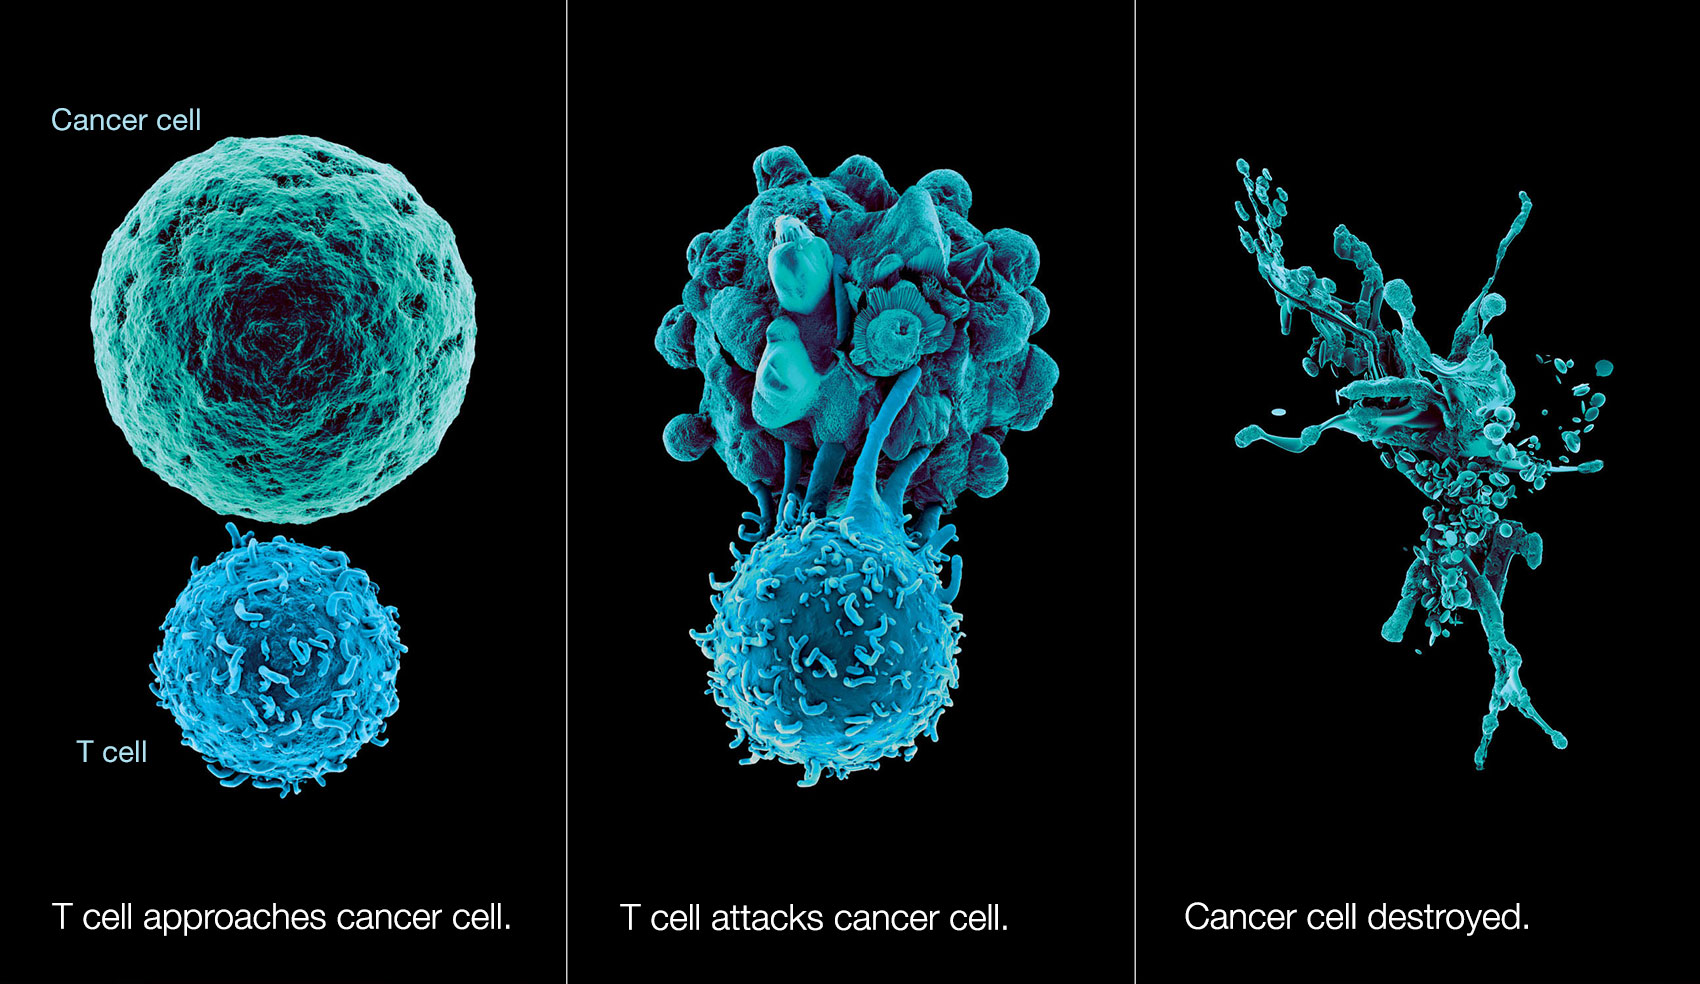
\includegraphics[width=0.85\textwidth]{img/neoantigen/tcell}
		\caption{Ejemplo de como una célula T destruye células del cancer \cite{nortshore2022}.}
	\end{figure}		
\end{frame}
%-------------------------------------------------------
%-------------------------------------------------------

%-------------------------------------------------------
%-------------------------------------------------------
\begin{frame}{Inmunoterapia del Cáncer}{Neo antígenos}		
	\begin{block}{}
		Es una \textbf{proteína} que se forma en las células de Cáncer cuando ocurre mutaciones en el DNA, cumplen un rol importante al \textbf{estimular una respuesta inmune} \cite{NCIdictionary2022, borden2022cancer}.
	\end{block} 
	\begin{block}{}
		En la actualidad hay varios métodos para detectar a predecir neo antígenos, pero \textbf{solo una pequeña cantidad de ellos} logran estimular al sistema inmune \cite{chen2021challenges, hao2021improvement}.
	\end{block}
\end{frame}
%-------------------------------------------------------
%-------------------------------------------------------

%-------------------------------------------------------
%-------------------------------------------------------
\begin{frame}{Inmunoterapia del Cáncer}{Generación de vacunas}	
	\begin{figure}
		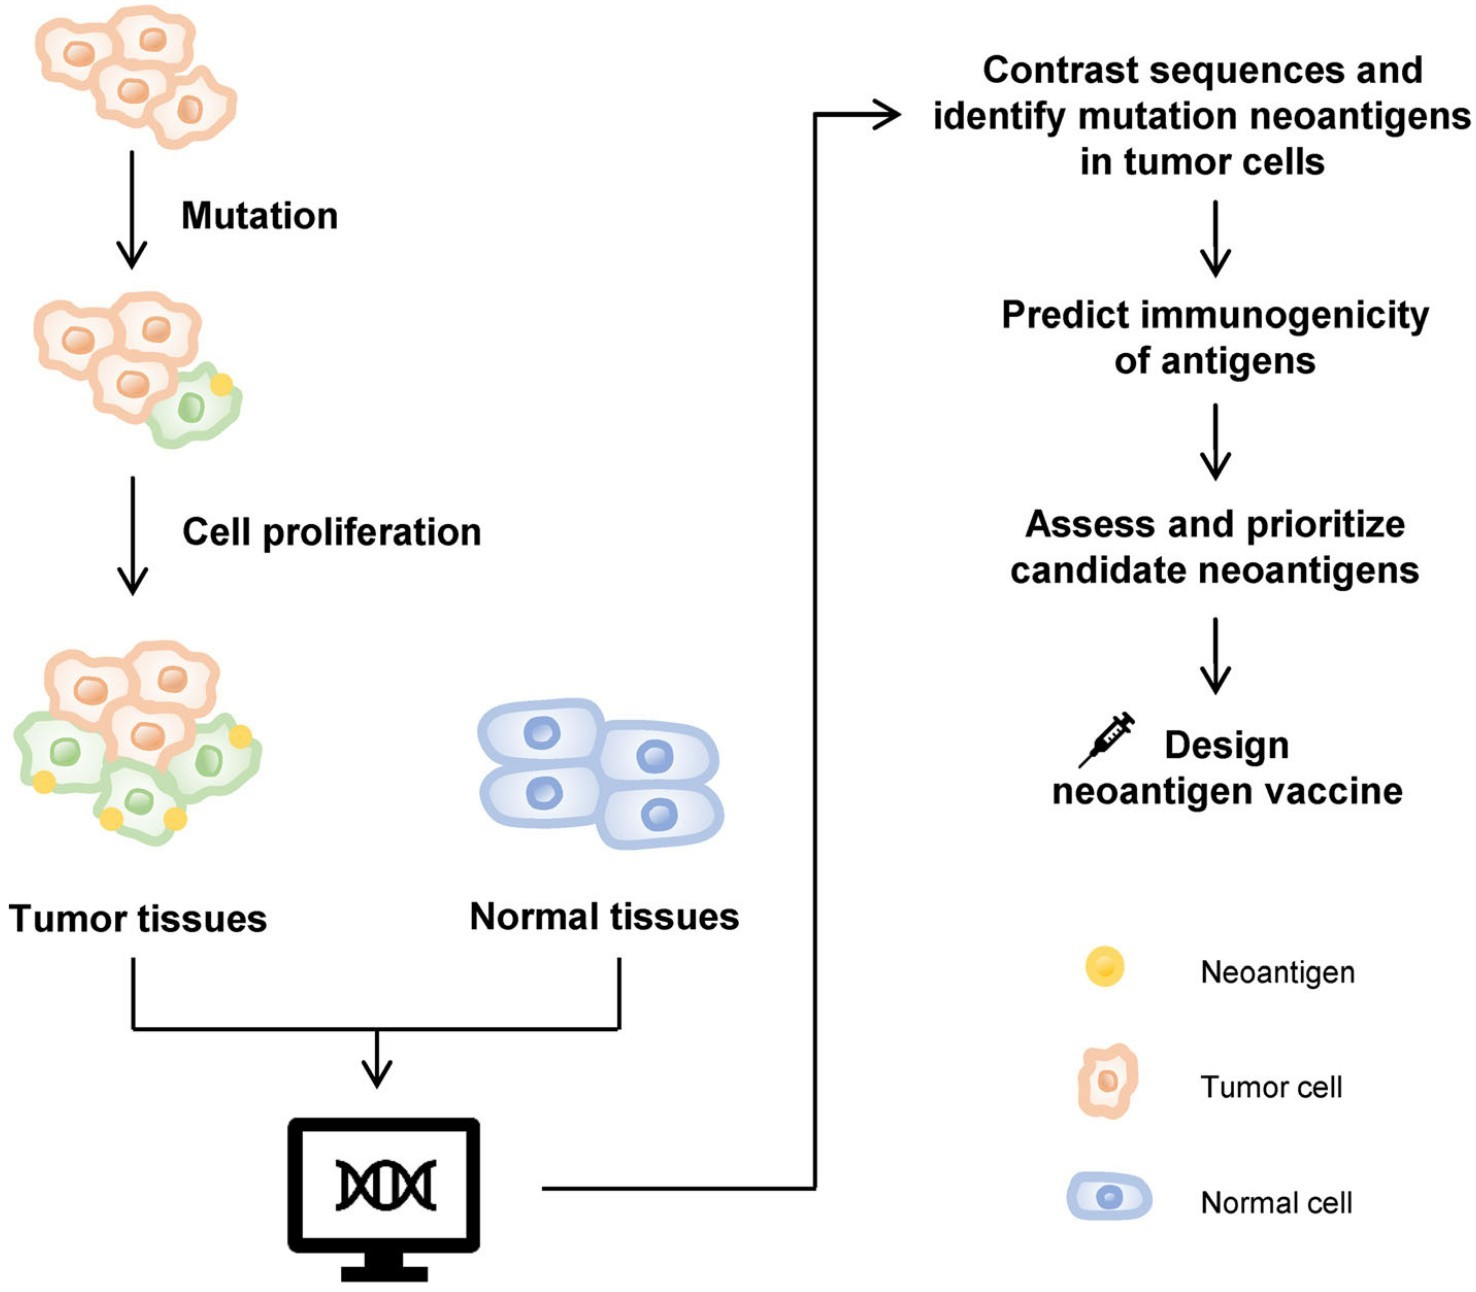
\includegraphics[width=0.6\textwidth]{img/neoantigen/process}
		\caption{Proceso para la generación de vacunas personalizadas \cite{peng2019neoantigen}.}
	\end{figure}		
\end{frame}
%-------------------------------------------------------
%-------------------------------------------------------


%-------------------------------------------------------
%-------------------------------------------------------
\begin{frame}{MHC-I}{}		
	\begin{figure}[H]
		\centering
		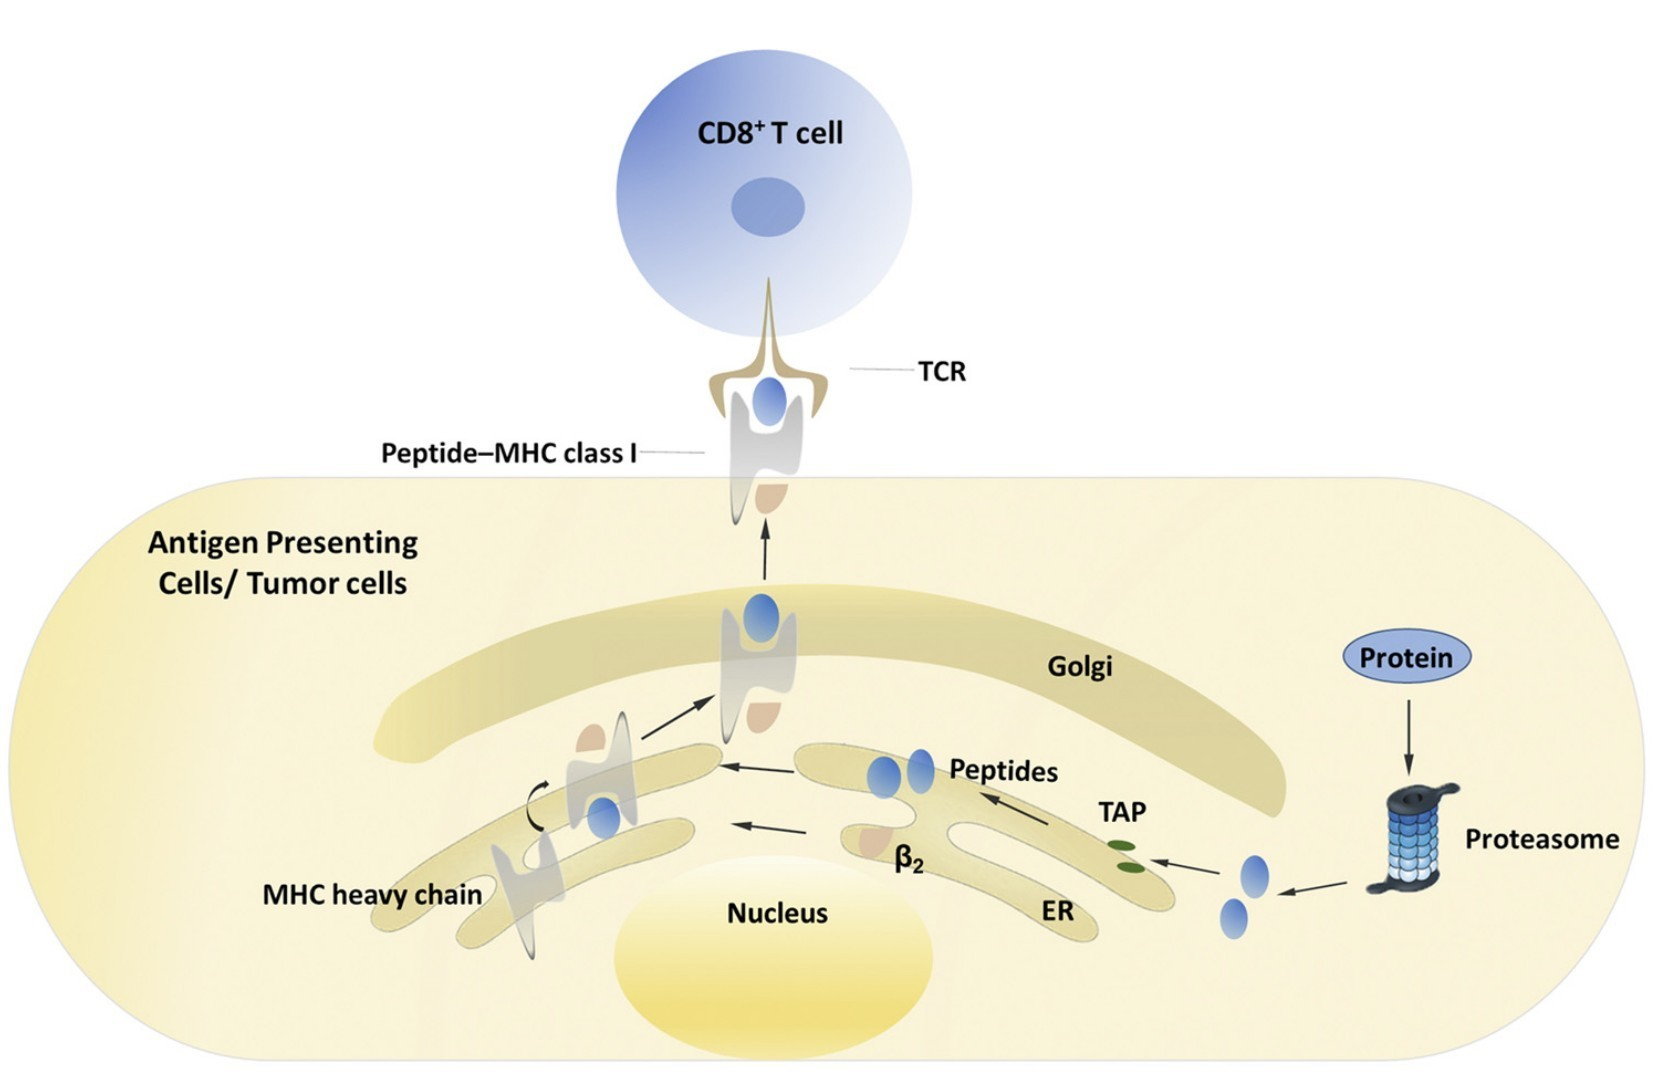
\includegraphics[width=0.9\textwidth]{img/neoantigen/mhc1.jpg}
		\caption{Presentación de antígenos por MHC-I. Fuente: \cite{zhang2019application}}
		\label{fig:mhc1}
	\end{figure}	
\end{frame}
%-------------------------------------------------------
%-------------------------------------------------------



%%%%%%%%%%%%%%%%%%%%%%%%%%%%%%%%%%%%%%%%%%%%%%%%%%%%%%%%%%%%%%%%%%%%%%%%%%%%%%%%%%%%%%%%%%%%%%%%%%%%%%%%%%%%%%%%
%%%%%%%%%%%%%%%%%%%%%%%%%%%%%%%%%%%%%%%%%%%%%%%%%%%%%%%%%%%%%%%%%%%%%%%%%%%%%%%%%%%%%%%%%%%%%%%%%%%%%%%%%%%%%%%%
%%%%%%%%%%%%%%%%%%%%%%%%%%%%%%%%%%%%%%%%%%%%%%%%%%%%%%%%%%%%%%%%%%%%%%%%%%%%%%%%%%%%%%%%%%%%%%%%%%%%%%%%%%%%%%%%
\subsection{Problema y Objetivos}
%%%%%%%%%%%%%%%%%%%%%%%%%%%%%%%%%%%%%%%%%%%%%%%%%%%%%%%%%%%%%%%%%%%%%%%%%%%%%%%%%%%%%%%%%%%%%%%%%%%%%%%%%%%%%%%%
%%%%%%%%%%%%%%%%%%%%%%%%%%%%%%%%%%%%%%%%%%%%%%%%%%%%%%%%%%%%%%%%%%%%%%%%%%%%%%%%%%%%%%%%%%%%%%%%%%%%%%%%%%%%%%%%
%%%%%%%%%%%%%%%%%%%%%%%%%%%%%%%%%%%%%%%%%%%%%%%%%%%%%%%%%%%%%%%%%%%%%%%%%%%%%%%%%%%%%%%%%%%%%%%%%%%%%%%%%%%%%%%%

%-------------------------------------------------------
%-------------------------------------------------------
\begin{frame}{Motivación}{}	

\begin{block}{}
	El cáncer representa el mayor problema de salud mundial, pero lamentablemente los métodos basados en cirugías, radioterapias, quimioterapias tienen baja efectividad \cite{peng2019neoantigen}.
\end{block}	

\begin{block}{}
	La inmunoterapia del cáncer es una alternativa para el desarrollo de vacunas personalizadas, pero este proceso depende de una correcta detección de neo antígenos \cite{de2020neoantigen, peng2019neoantigen}.
\end{block}

\end{frame}
%-------------------------------------------------------
%-------------------------------------------------------



%-------------------------------------------------------
%-------------------------------------------------------
\begin{frame}{Problema}{}
	
\begin{block}{}
	\textbf{Menos del 3\%} de los neoantígenos detectados logran activar a las células T (sistema inmune) \cite{de2020neoantigen}. 
\end{block}
	
\end{frame}
%-------------------------------------------------------
%-------------------------------------------------------

%-------------------------------------------------------
%-------------------------------------------------------
\begin{frame}{Objetivos}{Objetivo general}	
	\begin{block}{Objetivo general}
		Desarrollar una revisión sistemática de métodos que utilizan \textit{deep learning} para la detección de neo antígenos.
	\end{block}	
\end{frame}
%-------------------------------------------------------
%-------------------------------------------------------


%%%%%%%%%%%%%%%%%%%%%%%%%%%%%%%%%%%%%%%%%%%%%%%%%%%%%%%%%%%%%%%%%%%%%%%%%%%%%%%%%%%%%%%%%%%%%%%%%%%%%%%%%%%%%%%%
%%%%%%%%%%%%%%%%%%%%%%%%%%%%%%%%%%%%%%%%%%%%%%%%%%%%%%%%%%%%%%%%%%%%%%%%%%%%%%%%%%%%%%
\section{Revisión Sistemática}
%%%%%%%%%%%%%%%%%%%%%%%%%%%%%%%%%%%%%%%%%%%%%%%%%%%%%%%%%%%%%%%%%%%%%%%%%%%%%%%%%%%%%%%%%%%%%%%%%%%%%%%%%%%%%%%%
%%%%%%%%%%%%%%%%%%%%%%%%%%%%%%%%%%%%%%%%%%%%%%%%%%%%%%%%%%%%%%%%%%%%%%%%%%%%%%%%%%%%%%


%%%%%%%%%%%%%%%%%%%%%%%%%%%%%%%%%%%%%%%%%%%%%%%%%%%%%%%%%%%%%%%%%%%%%%%%%%%%%%%%%%%%%%%%%%%%%%%%%%%%%%%%%%%%%%%%
%%%%%%%%%%%%%%%%%%%%%%%%%%%%%%%%%%%%%%%%%%%%%%%%%%%%%%%%%%%%%%%%%%%%%%%%%%%%%%%%%%%%%%
\subsection{Metodología}
%%%%%%%%%%%%%%%%%%%%%%%%%%%%%%%%%%%%%%%%%%%%%%%%%%%%%%%%%%%%%%%%%%%%%%%%%%%%%%%%%%%%%%%%%%%%%%%%%%%%%%%%%%%%%%%%
%%%%%%%%%%%%%%%%%%%%%%%%%%%%%%%%%%%%%%%%%%%%%%%%%%%%%%%%%%%%%%%%%%%%%%%%%%%%%%%%%%%%%%


%-------------------------------------------------------
%-------------------------------------------------------
\begin{frame}{Revisión Sistemática}{Preguntas de investigación}
	
	\begin{table}[h]
		\begin{center}
			\caption{Research questions used in SLR.}
			\label{tab:questions}
			\setlength{\tabcolsep}{0.5em} % for the horizontal padding
			{\renewcommand{\arraystretch}{1.4}% for the vertical padding
				\begin{tabular}{p{8.5cm}}
					\textbf{Preguntas de investigación} \\ \hline
					\textbf{Q1}. Como se utilizan las técnicas de \textit{deep learning} para la detección de neo antígenos?\\
					\textbf{Q2}. Que tipos de datos y pre procesamiento es utilizado en la detección de ne antígenos?\\
					\textbf{Q3}. Que bases de datos son utilizadas en la detección de neo antígenos?\\
					\textbf{Q4}. Que método basado en \textit{deep learning} tiene los mejores resultados?   \\		
				\end{tabular}
			}
		\end{center}
	\end{table}

\end{frame}
%-------------------------------------------------------
%-------------------------------------------------------

%-------------------------------------------------------
%-------------------------------------------------------
\begin{frame}{Revisión Sistemática}{Metodología}
	
	\begin{table}[H]
		\begin{center}
			\caption{Cadenas de busqueda utilizadas en la RSL.}
			\label{tab:key_words}
			\setlength{\tabcolsep}{0.5em} % for the horizontal padding
			{\renewcommand{\arraystretch}{1.4}% for the vertical padding
				\begin{tabular}{p{10cm}}
					\textbf{Cadena de busqueda} \\ \hline
					neoantigen  AND (detection OR pipeline) AND deep learning                                                                               \\
					(MHC OR HLA) AND binding  AND deep learning                                                                                             \\				
					(MHC-I OR MHC-II OR MHC OR HLA) AND (peptide OR epitope) AND ( binding OR affinity OR prediction OR detection OR presentation)          \\
					TCR interaction prediction                                                                                                              \\		
				\end{tabular}
			}
		\end{center}
	\end{table}
\end{frame}
%-------------------------------------------------------
%-------------------------------------------------------


%-------------------------------------------------------
%-------------------------------------------------------
\begin{frame}{Revisión Sistemática}{Metodología}
	
	\begin{table}[H]
		\centering
		\begin{center}
			\caption{Bases de datos utilizadas en la RSL.}
			\label{tab:bd_RSL}
			\setlength{\tabcolsep}{0.5em} % for the horizontal padding
			{\renewcommand{\arraystretch}{1.2}% for the vertical padding
				\begin{tabular}{p{3cm}}
					\textbf{Bases de datos} \\ \hline
					IEEE Xplore                                                                               \\
					Science Direct \\				
					Springer          \\
					ACM Digital Library                                                                                                             \\	
					PubMed \\ 
					BioRxiv \\ 	
				\end{tabular}
			}
		\end{center}
	\end{table}
	
\end{frame}
%-------------------------------------------------------
%-------------------------------------------------------



%-------------------------------------------------------
%-------------------------------------------------------
\begin{frame}{Revisión Sistemática}{Metodología}
	
	\begin{table}[H]
		\begin{center}
			\caption{Criterios de inclusión y exclusión de artículos utilizados en la RSL.}
			\label{tab:criterios}
			\setlength{\tabcolsep}{0.5em} % for the horizontal padding
			{\renewcommand{\arraystretch}{1.2}% for the vertical padding
				\begin{tabular}{p{5cm}p{5cm}}
					\textbf{Criterios de inclusión}                                                   & \textbf{Criterios de exclusión}                                                           \\ \hline
					Artículos con categoría ERA (A, B o C) si son conferencias y Journals Q1, Q2 o Q3. & Trabajos de baja calidad, que no esten rankeados.                                      \\
					Sobre \textit{deep learning}                \\
					La metodología es detallada.                                                                                                               &                                                                                                        \\
					Tiene repositorio de código fuente y base de datos (deseable).                                          &                                                                                                        \\
					
				\end{tabular}
			}
		\end{center}
	\end{table}
	
\end{frame}
%-------------------------------------------------------
%-------------------------------------------------------






%-------------------------------------------------------
%-------------------------------------------------------
\begin{frame}{Revisión Sistemática}{Metodología}
	
	\begin{table}[H]
		\begin{center}
			\caption{Cantidad de artículos encontrados y seleccionados según los criterios de inclusión y exclusión en la RSL.}
			\label{tab:number_papers}
			\setlength{\tabcolsep}{0.5em} % for the horizontal padding
			{\renewcommand{\arraystretch}{1.2}% for the vertical padding
				\begin{tabular}{ccc}
					\textbf{Año} & \textbf{Artículos encontrados} & \textbf{Artículos seleccionados}\\ \hline
					2018 & 57 & 21 \\
					2019 & 72 & 31 \\
					2020 & 86 & 29 \\
					2021 & 61 & 34 \\
					2022 & 58 & 19 \\ \hline
					Total & \textbf{334} & \textbf{134} \\
				\end{tabular}
			}
		\end{center}
	\end{table}
	
\end{frame}
%-------------------------------------------------------
%-------------------------------------------------------

%%%%%%%%%%%%%%%%%%%%%%%%%%%%%%%%%%%%%%%%%%%%%%%%%%%%%%%%%%%%%%%%%%%%%%%%%%%%%%%%%%%%%%%%%%%%%%%%%%%%%%%%%%%%%%%%
%%%%%%%%%%%%%%%%%%%%%%%%%%%%%%%%%%%%%%%%%%%%%%%%%%%%%%%%%%%%%%%%%%%%%%%%%%%%%%%%%%%%%%
\subsection{Resultados}
%%%%%%%%%%%%%%%%%%%%%%%%%%%%%%%%%%%%%%%%%%%%%%%%%%%%%%%%%%%%%%%%%%%%%%%%%%%%%%%%%%%%%%%%%%%%%%%%%%%%%%%%%%%%%%%%
%%%%%%%%%%%%%%%%%%%%%%%%%%%%%%%%%%%%%%%%%%%%%%%%%%%%%%%%%%%%%%%%%%%%%%%%%%%%%%%%%%%%%%
%-------------------------------------------------------
%-------------------------------------------------------
\begin{frame}{Revisión Sistemática}{Convolutional Neural Networks}
	
	\fontsize{8pt}{5pt}\selectfont
	
	\begin{table}[]
		\centering
		\caption{List of research since 2018 that uses CNNs for peptide-MHC binding and presentation.}
		\setlength{\tabcolsep}{0.5em} % for the horizontal padding
		{\renewcommand{\arraystretch}{2}% for the vertical padding
			\begin{tabular}{p{0.6cm}p{0.6cm}p{1.5cm}p{2cm}p{0.6cm}p{2.7cm}}
				\textbf{Year} & \textbf{Ref.}                              & \textbf{Approach}        & \textbf{Name} & \textbf{MHC} & \textbf{Encoding}                                                                                                                                                                                   \\ \hline
				
				2022 &	\cite{you2022deepmhcii}	& pMHC(b) &	DeepMHCII &	 II &	PFR \\
				
				2021          & \cite{li2021deepimmuno}   & pMHC(b)      & DeepImmuno    &  I        & AAindex1                                                \\
				2021          & \cite{lang2021neofox}     & pMHC(p) & APPM          &  I        & One-hot                                                                          \\
				2021          & \cite{lee2021connecting}  & pMHC(p) & MHCfovea      &  I        & One-hot                                                                                                      \\
				2021          & \cite{junet2021cnn}       & pMHC(b)      & CNN-PepPred   &  II       & BLOSUM     \\
				
				2020          & \cite{pei2020iconmhc}     & pMHC(b)      & IConMHC       & I        & PCA and AAindex3        \\
				2020          & \cite{saxena2020onionmhc} & pMHC(b)      & OnionMHC      & I        & BLOSUM and structural features                                                                  \\
				2020          & \cite{ng3704016minerva}   & pMHC(p) & MINERVA       & I        & Physicochemical properties                                                           \\
				2019          & \cite{zhao2019peptide}    & pMHC(b)      & CNN-NF        & I        & Sequence, Hydropathy, Polarity, Length                    \\
				2019          & \cite{liu2019deepseqpan}  & pMHC(b)      & DeepSeqPan    & I        & One-hot                                          \\
				2018          & \cite{han2018deep}        & pMHC(b)      & ConvMHC       & I        & Contact side HLA.peptide                                                                                 
			\end{tabular}
		}
	\end{table}	
\end{frame}
%-------------------------------------------------------
%-------------------------------------------------------


%-------------------------------------------------------
%-------------------------------------------------------
\begin{frame}{Revisión Sistemática}{Convolutional Neural Networks}
	
	\fontsize{8pt}{5pt}\selectfont
	
	\begin{table}[]
		\centering
		\caption{List of research since 2018 that uses CNNs s with RNN or attention mechanisms for peptide-MHC binding and presentation. MHCherryPan uses CNN with RNN, the other uses CNN witn Attention mechanims.}		
		\setlength{\tabcolsep}{0.5em} % for the horizontal padding
		{\renewcommand{\arraystretch}{2}% for the vertical padding
			\begin{tabular}{p{0.6cm}p{0.6cm}p{1.5cm}p{2cm}p{0.6cm}p{2.7cm}}
				\textbf{Year} & \textbf{Ref.}                              & \textbf{Approach}   & \textbf{Name}    & \textbf{MHC} & \textbf{Encoding}                                           \\ \hline
				2021          & \cite{yang2021deepnetbim} & pMHC(b) & DeepNetBim       & I        & BLOSUM              \\
				
				2021          & \cite{jin2021deep}        & pMHC(b) & Deep Attention Pan & I        & BLOSUM                    \\
				
				2019          & \cite{hu2019acme}         & pMHC(b) & ACME             & I        & BLOSUM      \\
				
				2020          & \cite{xie2020mhcherrypan} & pMHC(b) & MHCherryPan      & I        & BLOSUM          
			\end{tabular}
		}
	\end{table}	
\end{frame}
%-------------------------------------------------------
%-------------------------------------------------------


%-------------------------------------------------------
%-------------------------------------------------------
\begin{frame}{Revisión Sistemática}{Recurrent Neural Networks}
	
	\fontsize{8pt}{5pt}\selectfont
	
	\begin{table}[]
		\centering
		\caption{List of research since 2018 that uses RNNs for peptide-MHC binding and presentation. MATHLA, DeepSeqPanII and DeepHLApan uses RNN with attention mechanims, meanwhile the other focus on GRU and LSTM.}		
		\setlength{\tabcolsep}{0.5em} % for the horizontal padding
		{\renewcommand{\arraystretch}{2}% for the vertical padding
			\begin{tabular}{p{0.6cm}p{0.6cm}p{1.5cm}p{2cm}p{0.6cm}p{2.7cm}}
				\textbf{Year} & \textbf{Ref.}                               & \textbf{Approach}   & \textbf{Name} & \textbf{MHC} & \textbf{Encoding}                                                                                                                                                                                                                         \\ \hline
				2021          & \cite{ye2021mathla}        & pMHC(b) & MATHLA        & I        & BLOSUM                      \\
				
				2021          & \cite{liu2021deepseqpanii} & pMHC(b)                     & DeepSeqPanII                      & II       & One-hot  and BLOSUM                                                    \\
				
				2021          & \cite{heng2021simple}      & pMHC(b)                     & GRU-based RNN                     & II       & Embeding layer                                                        \\
				
				2021          & \cite{jiang2021predicting} & pMHC(b)                     & BVLSTM-MHC                        & I        & One-hot  and BLOSUM                                                                        \\
				
				2020          & \cite{shao2020high}        & pMHC(b)                     & MHCnuggets                        & I, II & One-hot                \\
				
				2019          & \cite{wu2019deephlapan}    & pMHC(b)                     & DeepHLApan                        & I        & One-hot                     
			\end{tabular}
		}
	\end{table}	
\end{frame}
%-------------------------------------------------------
%-------------------------------------------------------



%-------------------------------------------------------
%-------------------------------------------------------
\begin{frame}{Revisión Sistemática}{Transformers}
	
	\fontsize{8pt}{5pt}\selectfont
	
	\begin{table}[]
		\centering
		\caption{List of research since 2018 that uses Transformers (self-attention) for peptide-MHC binding and presentation.}		
		\setlength{\tabcolsep}{0.5em} % for the horizontal padding
		{\renewcommand{\arraystretch}{2}% for the vertical padding
			\begin{tabular}{p{0.6cm}p{0.6cm}p{1.5cm}p{2cm}p{0.6cm}p{2.7cm}}
				\textbf{Year} & \textbf{Ref.}                                  & \textbf{Approach}        & \textbf{Name} & \textbf{MHC} & \textbf{Encoding}                                                                                                                                                                                                         \\ \hline
				2022          & \cite{wang2022mhcroberta}     & pMHC(b)      & MHCRoBERTa    & I        & Tokenized from a pre-trained model               \\
				2022          & \cite{chu2022transformer}     & pMHC(b)      & TransPHLA     & I        & Character embedding model           \\
				2021          & \cite{cheng2021bertmhc}       & pMHC(b)      & BERTMHC       & II       & Embeding layer                           \\
				2021          & \cite{gasser2021interpreting} & pMHC(p) & ImmunoBERT    & I        & Embeding layer             
			\end{tabular}
		}
	\end{table}	
\end{frame}
%-------------------------------------------------------
%-------------------------------------------------------



%-------------------------------------------------------
%-------------------------------------------------------
\begin{frame}{Revisión Sistemática}{Bases de datos}
	
	\fontsize{7pt}{5pt}\selectfont
	
	\begin{table}[]
		\centering
		\caption{Public databases of \textit{pMHC binding}, \textit{pMHC presentation}, pMHC-TCR interaction, and 3D structures of proteins.}		
		\setlength{\tabcolsep}{0.5em} % for the horizontal padding
		{\renewcommand{\arraystretch}{2}% for the vertical padding
			\begin{tabular}{p{1.7cm}p{1.2cm}p{6.5cm}}
				\textbf{Name} & \textbf{Year ref.}                                                                & \textbf{Description}                                                                                                                                                                                      \\ \hline
				VDJdb           & 2018 \cite{shugay2018vdjdb}& TCR binding to pMHC, contains 5491 samples.                                                                                                                                           \\
				IEDB            & 2018 \cite{vita2019immune}                                           & The bigger database, contains information \textit{T-cell epitopes}                                                                                               \\
				TSNAdb          & 2018 \cite{wu2018tsnadb}                                             & It contains 7748 samples of mutations and HLA of 16 types of cancer.                                                                                                                           \\
				NeoPeptide      & 2019 \cite{zhou2019neopeptide}                                       & It contains samples of neoantigens resulting from somatic mutations and related items. 1818137 epitopes of more than 36000 neoantigens.
				\\
				pHLA3D          & 2019 \cite{e2019phla3d}                                              &
				Presents 106 3D structures of the alpha, $beta 2M$ chains, and peptides of HLA-I molecules                                                                                                            \\
				dbPepNeo        & 2020 \cite{tan2020dbpepneo}                                          & It has validated samples of the \textit{peptide-MHC} bond, from MS. It contains 407794 low-quality samples, 247 medium-quality, and 295 high-quality samples.
				\\
				dbPepNeo2.0    & 2022 \cite{lu2022dbpepneo2}                                          &
				It gathers a list of neoantigens and HLA molecules. It presents 801 high-quality and 842,289 poor-quality HLAs. Also, 55 class II neoantigens and 630 TCR-bound neo antigens.
				\\
				IntroSpect      & 2022 \cite{zhang2022introspect}                                      & Tool for building databases on \textit{peptide-MHC binding}. It uses data from \textit{Mass Spectrometry}.   \\
				
				IPD-IMGT/HLA & 2022 \cite{robinson2020ipd}    &    With 25000 MHC molecules and 45 alleles.                                                                
			\end{tabular}
		}
	\end{table}	
\end{frame}
%-------------------------------------------------------
%-------------------------------------------------------


%-------------------------------------------------------
%-------------------------------------------------------
\begin{frame}{Revisión Sistemática}{Pipelines}
	
	\fontsize{7pt}{5pt}\selectfont
	
	\begin{table}[]
		\centering
		\caption{List of \textit{pipelines} since 2018 for the detection of neoantigens.}		
		\setlength{\tabcolsep}{0.5em} % for the horizontal padding
		{\renewcommand{\arraystretch}{2}% for the vertical padding
			\begin{tabular}{lp{1.2cm}p{2.5cm}p{2.5cm}}
				\textbf{Name} & \textbf{Year ref.}                                  & \textbf{Input}                                         & \textbf{Output}                                     \\ \hline
				Neopepsee       & 2018 \cite{kim2018neopepsee}           & RNA-seq, somatic mutations (VCF), HLA type (optional) & Neoantigens and gene expression levels   \\ 
				PGV Pipeline    & 2018 \cite{rubinsteyn2018computational}& DNA-seq                                                  & Neoantigens                                       \\
				ScanNeo         & 2019 \cite{wang2019scanneo}            & RNA-seq                                                  & Neoantigens                                       \\
				NeoPredPipe     & 2019 \cite{schenck2019neopredpipe}     & Mutations (VCF) y HLA type                           & Neoantigens and variant annotation              \\
				pVACtools       & 2020 \cite{hundal2020pvactools}        & Mutations (VCF)                                         & Neoantigens                                       \\
				ProGeo-neo      & 2020 \cite{li2020progeo}               & RNA-seq y somatic mutations (VCF)                        & Neoantigens                                       \\
				Neoepiscope     & 2020 \cite{wood2020neoepiscope}        & Somatic mutations (VCF) and BAM files                  & Neoantigens and mutations                          \\
				NeoANT-HILL     & 2020 \cite{coelho2020neoant}           & RNA-seq y somatic mutations (VCF)                        & Neoantigens and gene expression levels \\
				NAP-CNB         & 2021 \cite{wert2021predicting}         & RNA-seq                                                  & Neoantigens                                       \\
				
				PEPPRMINT         & 2021 \cite{zhou2021prioritizing}         & DNA-seq                                                  & Neoantigens                                        \\
				
				Valid-NEO       & 2022 \cite{terai2022valid}             & Somatic mutations (VCF), HLA type (optional)          & Neoantigens                                       
			\end{tabular}
		}
	\end{table}	
\end{frame}
%-------------------------------------------------------
%-------------------------------------------------------




%%%%%%%%%%%%%%%%%%%%%%%%%%%%%%%%%%%%%%%%%%%%%%%%%%%%%%%%%%%%%%%%%%%%%%%%%%%%%%%%%%%%%%%%%%%%%%%%%%%%%%%%%%%%%%%%
%%%%%%%%%%%%%%%%%%%%%%%%%%%%%%%%%%%%%%%%%%%%%%%%%%%%%%%%%%%%%%%%%%%%%%%%%%%%%%%%%%%%%%
\section{Discusión}
%%%%%%%%%%%%%%%%%%%%%%%%%%%%%%%%%%%%%%%%%%%%%%%%%%%%%%%%%%%%%%%%%%%%%%%%%%%%%%%%%%%%%%%%%%%%%%%%%%%%%%%%%%%%%%%%
%%%%%%%%%%%%%%%%%%%%%%%%%%%%%%%%%%%%%%%%%%%%%%%%%%%%%%%%%%%%%%%%%%%%%%%%%%%%%%%%%%%%%%


%-------------------------------------------------------
%-------------------------------------------------------
\begin{frame}{Discusión}{}
	\begin{block}{Como se utilizan las técnicas de \textit{deep learning} para la detección de neo antígenos?}
		 La detección de neo antígenos es visto como un problema de clasificación binaría.
	\end{block}

	\centering
	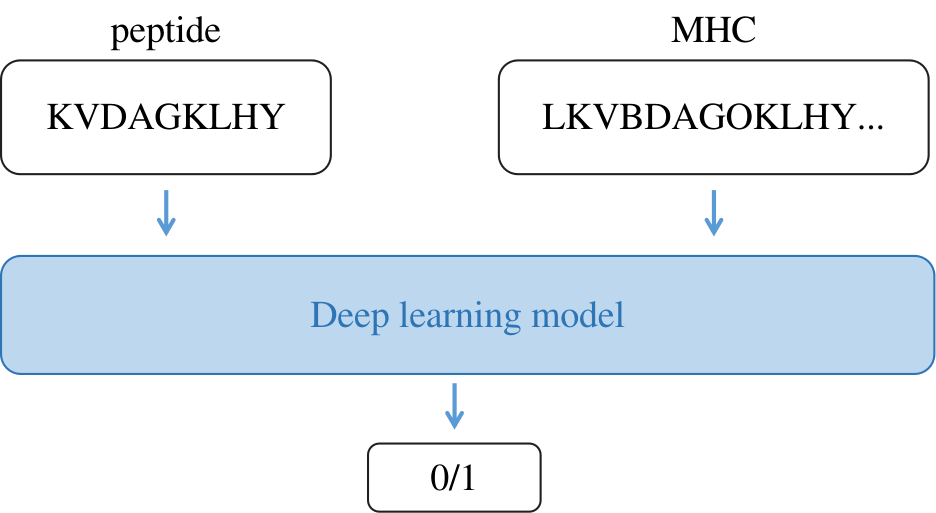
\includegraphics[width=0.7\textwidth]{img/neoantigen/q1}
	
\end{frame}
%-------------------------------------------------------
%-------------------------------------------------------

%-------------------------------------------------------
%-------------------------------------------------------
\begin{frame}{Discusión}{}
	\begin{block}{Que tipos de datos y pre procesamiento es utilizado en la detección de ne antígenos?}
		Se consideran las cadenas de aminoacidos, como pre procesamiento se utiliza \textit{one-hot encoding} y \textit{BLOSUM}.
	\end{block}
	
	\centering
\begin{columns}	
		
	\begin{column}{0.48\textwidth}
		\centering
		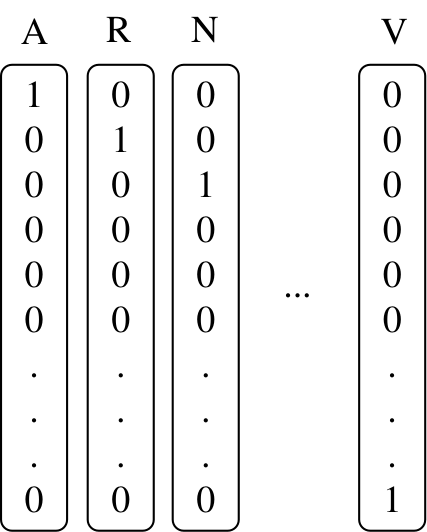
\includegraphics[width=0.5\textwidth]{img/neoantigen/onehot}
	\end{column}
	
	\begin{column}{0.48\textwidth}
		\centering
		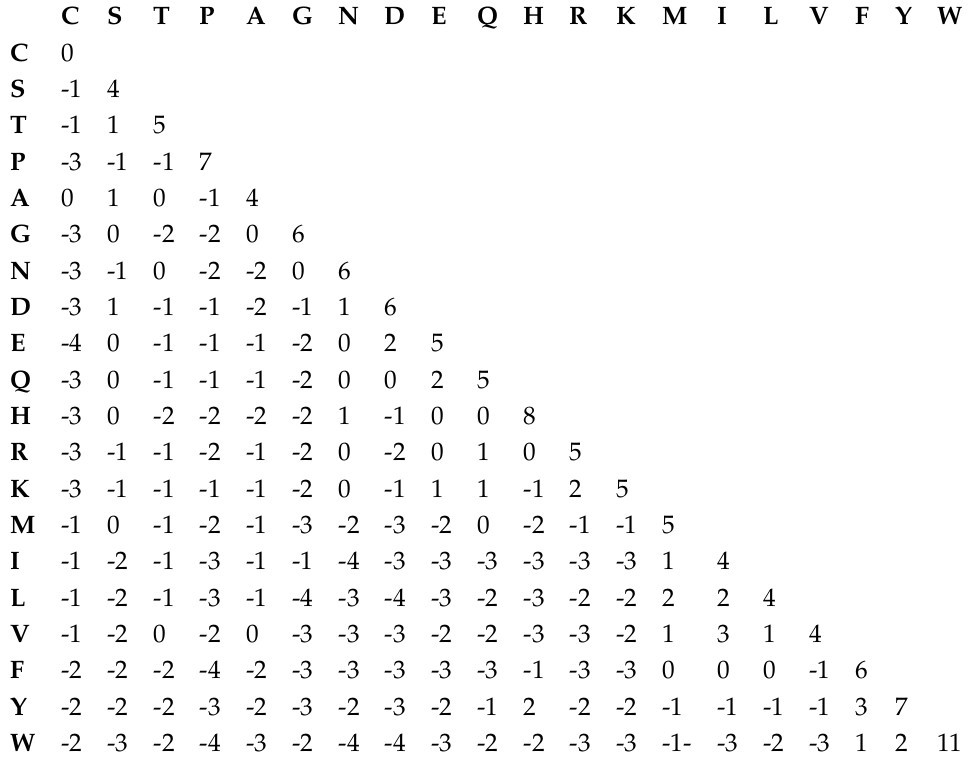
\includegraphics[width=0.9\textwidth]{img/neoantigen/blosum}
	\end{column}
\end{columns}		
	

	
\end{frame}
%-------------------------------------------------------
%-------------------------------------------------------

%-------------------------------------------------------
%-------------------------------------------------------
\begin{frame}{Discusión}{}
	\begin{block}{Que bases de datos son utilizadas en la detección de neo antígenos?}
		Tabla descrita anteriormente.
	\end{block}	
\end{frame}
%-------------------------------------------------------
%-------------------------------------------------------

%-------------------------------------------------------
%-------------------------------------------------------
\begin{frame}{Discusión}{Bases de datos}
	
	\fontsize{7pt}{5pt}\selectfont
	
	\begin{table}[]
		\centering
				
		\setlength{\tabcolsep}{0.5em} % for the horizontal padding
		{\renewcommand{\arraystretch}{2}% for the vertical padding
			\begin{tabular}{p{1.7cm}p{1.2cm}p{6.5cm}}
				\textbf{Name} & \textbf{Year ref.}                                                                & \textbf{Description}                                                                                                                                                                                      \\ \hline
				VDJdb           & 2018 \cite{shugay2018vdjdb}& TCR binding to pMHC, contains 5491 samples.                                                                                                                                           \\
				IEDB            & 2018 \cite{vita2019immune}                                           & The bigger database, contains information \textit{T-cell epitopes}                                                                                               \\
				TSNAdb          & 2018 \cite{wu2018tsnadb}                                             & It contains 7748 samples of mutations and HLA of 16 types of cancer.                                                                                                                           \\
				NeoPeptide      & 2019 \cite{zhou2019neopeptide}                                       & It contains samples of neoantigens resulting from somatic mutations and related items. 1818137 epitopes of more than 36000 neoantigens.
				\\
				pHLA3D          & 2019 \cite{e2019phla3d}                                              &
				Presents 106 3D structures of the alpha, $beta 2M$ chains, and peptides of HLA-I molecules                                                                                                            \\
				dbPepNeo        & 2020 \cite{tan2020dbpepneo}                                          & It has validated samples of the \textit{peptide-MHC} bond, from MS. It contains 407794 low-quality samples, 247 medium-quality, and 295 high-quality samples.
				\\
				dbPepNeo2.0    & 2022 \cite{lu2022dbpepneo2}                                          &
				It gathers a list of neoantigens and HLA molecules. It presents 801 high-quality and 842,289 poor-quality HLAs. Also, 55 class II neoantigens and 630 TCR-bound neo antigens.
				\\
				IntroSpect      & 2022 \cite{zhang2022introspect}                                      & Tool for building databases on \textit{peptide-MHC binding}. It uses data from \textit{Mass Spectrometry}.   \\
				
				IPD-IMGT/HLA & 2022 \cite{robinson2020ipd}    &    With 25000 MHC molecules and 45 alleles.                                                                
			\end{tabular}
		}
	\end{table}	
\end{frame}
%-------------------------------------------------------
%-------------------------------------------------------


%-------------------------------------------------------
%-------------------------------------------------------
\begin{frame}{Discusión}{}
	\begin{block}{Que método basado en \textit{deep learning} tiene los mejores resultados? }
		
		\textbf{NetMHCpan4.1} es considerado el método con mejor desempeño. Pero, recientemente, \textbf{HLAB} \cite{zhang2022hlab} utilizado para \textit{pMHC-I binding prediction},  utiliza  BiLSTM, proBERT y \textit{transfer learning} de UniRef100 \cite{suzek2015uniref} y BFD \cite{steinegger2018clustering}; este modelo ha superado a NetMHCpan4.1. 
	\end{block}	
\end{frame}
%-------------------------------------------------------
%-------------------------------------------------------

%%%%%%%%%%%%%%%%%%%%%%%%%%%%%%%%%%%%%%%%%%%%%%%%%%%%%%%%%%%%%%%%%%%%%%%%%%%%%%%%%%%%%%%%%%%%%%%%%%%%%%%%%%%%%%%%
%%%%%%%%%%%%%%%%%%%%%%%%%%%%%%%%%%%%%%%%%%%%%%%%%%%%%%%%%%%%%%%%%%%%%%%%%%%%%%%%%%%%%%
\section{Trabajos futuros}
%%%%%%%%%%%%%%%%%%%%%%%%%%%%%%%%%%%%%%%%%%%%%%%%%%%%%%%%%%%%%%%%%%%%%%%%%%%%%%%%%%%%%%%%%%%%%%%%%%%%%%%%%%%%%%%%
%%%%%%%%%%%%%%%%%%%%%%%%%%%%%%%%%%%%%%%%%%%%%%%%%%%%%%%%%%%%%%%%%%%%%%%%%%%%%%%%%%%%%%


%\textbf{Q1}. Como se utilizan las técnicas de \textit{deep learning} para la detección de neo antígenos?\\
%\textbf{Q2}. Que tipos de datos y pre procesamiento es utilizado en la detección de ne antígenos?\\
%\textbf{Q3}. Que bases de datos son utilizadas en la detección de neo antígenos?\\
%\textbf{Q4}. Que método basado en \textit{deep learning} tiene los mejores resultados?   \\	

%-------------------------------------------------------
%-------------------------------------------------------
\begin{frame}{Trabajos futuros}{}
	\begin{block}{}
		Recientemente un trabajo \cite{hashemi2022improved} tambien propone el uso de \textit{transfer learning} pero de un modelo pre-entrenado con 250 millones de proteínas. Entonces, se plantea utilizar la propuesta de HLAB, aumentar la cantidad de muestras y evaluar los resultados.
	\end{block}
	
	\begin{block}{}
		Actualmente se cuenta con una base de datos de proteínas MHC \cite{e2019phla3d}, entonces utilizando AlphaFold de Google, se plantea predecir la estructura de varios péptidos y analizar el enlace péptido-MHC desde un punto de vista de la computación gráfica.	
	\end{block}
	
	
\end{frame}
%-------------------------------------------------------
%-------------------------------------------------------

%-------------------------------------------------------
%-------------------------------------------------------
\begin{frame}[allowframebreaks, noframenumbering]
	\frametitle{References}
	%\bibliographystyle{amsalpha}
	\bibliographystyle{IEEEtran}
	\bibliography{Bibliography.bib}
\end{frame}
%-------------------------------------------------------
%-------------------------------------------------------

%-------------------------------------------------------
%-------------------------------------------------------
\if\mycmd1 % MY THEME
\1{
	{\1
		\begin{frame}[plain,noframenumbering]
			%\finalpage{Thank you}
			\begin{figure}[]
				\centering
				
\includegraphics[width=\textwidth,height=0.7\textheight,keepaspectratio]{img/question.png}
				%\label{img:mot2}
				%\caption{Image example in 2 gray levels.}
			\end{figure}
	\end{frame}}
	\else % CS THEME
	\begin{frame}{Questions?}
		\begin{figure}[]
			\centering
			
\includegraphics[width=\textwidth,height=0.7\textheight,keepaspectratio]{img/question.png}
			%\label{img:mot2}
			%\caption{Image example in 2 gray levels.}
		\end{figure}
		
	\end{frame}
	\fi
	%-------------------------------------------------------
	%-------------------------------------------------------
	

\end{document}